% 'draft' mode can be used to speed up compilation
\documentclass[oneside,final]{report}
\usepackage{codespace}
% Draft watermark
% https://github.com/callegar/LaTeX-draftwatermark

% Encodings
\usepackage{gensymb,textcomp}
% Better tables
% Wide tables go to https://tex.stackexchange.com/q/332902
\usepackage{array,longtable,multicol,multirow,siunitx,tabularx}

% Better enum
\usepackage{enumitem}

% Graphics
\usepackage{caption,float}
\usepackage{multirow}
\usepackage{siunitx}
\usepackage{subcaption}
% Add options for figures, like max width, framing, etc.
\usepackage[export]{adjustbox}

% References
% Use \ref{} instead of \ref{}
\usepackage[nameinlink]{cleveref}
\usepackage{hyperref}

\usepackage[style=ieee]{biblatex}
\addbibresource{references.bib}

% --- TIẾNG VIỆT CHO CLEVEREF ---
% Định dạng cho \cref (chữ thường)
\crefname{section}{mục}{các mục}
\crefname{subsection}{tiểu mục}{các tiểu mục}
\crefname{figure}{hình}{các hình}
\crefname{table}{bảng}{các bảng}
\crefname{page}{trang}{các trang}
\crefname{equation}{phương trình}{các phương trình}
\crefname{lstlisting}{listing}{các listing} % Hoặc "đoạn mã" nếu muốn

% Định dạng cho \Cref (VIẾT HOA ĐẦU CÂU)
\Crefname{section}{Mục}{Các mục}
\Crefname{subsection}{Tiểu mục}{Các tiểu mục}
\Crefname{figure}{Hình}{Các hình}
\Crefname{table}{Bảng}{Các bảng}
\Crefname{page}{Trang}{Các trang}
\Crefname{equation}{Phương trình}{Các phương trình}
\Crefname{lstlisting}{Listing}{Các listing} % Hoặc "Đoạn mã"
% --- KẾT THÚC TIẾNG VIỆT CHO CLEVEREF ---
% FOR DEMONSTRATION PURPOSES, REMOVE IN PRODUCTION
\usepackage{mwe}

% Sub-preambles
% https://github.com/MartinScharrer/standalone

% Configurations
\coursename{CS105.P22 - Computer Graphics}
\reporttype{Báo cáo - Bài tập 4}
\title{\LARGE Tiểu luận Fractal}
\advisor{& \large ThS. Cáp Phạm Đình Thăng&}
\stuname{%
  & \large Lê Cảnh Nhật - 22521016 & \\
  & \large Tăng Nhất - 22521027 & \\
  & \large Thái Ngọc Quân - 22521189 & \\

}

% Allow page breaks inside align* environment
%\allowdisplaybreaks{}

% Makes a lot of things blue, avoid at all costs
%\everymath{\color{blue}}

% Set depth of numbering for counters
\AtBeginDocument{\counterwithin{lstlisting}{section}}

% Rename some sections
%\AtBeginDocument{\renewcommand*{\contentsname}{Contents}}
%\AtBeginDocument{\renewcommand*{\refname}{References}}
%\AtBeginDocument{\renewcommand*{\bibname}{References}}

% Custom commands
%\newcommand*\mean[1]{\bar{#1}}

\begin{document}
\coverpage%

%\section*{Member list \& Workload}
%\newcounter{memberrowno}
%\setcounter{memberrowno}{0}
%\begin{center}
%  \begin{tabular}{>{\stepcounter{memberrowno}\thememberrowno}llcc}
%    \toprule
%    \multicolumn{1}{c}{\textbf{No.}} & \textbf{Full name} & \textbf{Student ID} & \textbf{Contribution} \\
%    \midrule
%                                     & h                  & xxxxxxx             & 100\%                       \\
%                                     & h                  & xxxxxxx             & 100\%                       \\
%    \bottomrule
%  \end{tabular}
%\end{center}
%\clearpage

\tableofcontents
\listoffigures
\listoftables
\section{Nội dung}
\subsection{Tập Mandelbrot (Mandelbrot Set)}
Tập Mandelbrot~\cite{wiki:fractal,wiki:mandelbrot-set,enwiki:mandelbrot-set} là một tập hợp được đặt tên theo nhà toán học Benoit Mandelbrot, nó đã được nghiên cứu bởi nhiều nhà toán học và hình ảnh của nó có sức hấp dẫn không chỉ trong lĩnh vực toán học mà còn cả trong lĩnh vực nghệ thuật.
 Được mệnh danh là "Dấu vân tay của Chúa"~\cite{xavier2021thumbprint}, tập hợp này trở thành một ví dụ tiêu biểu cho cấu trúc phức tạao nên từ những quy tắc đơn giản và là một trong nhưng hình fractal nổi tiếng nhất.
Tập Mandelbrot là một tập hợp các điểm nằm trong mặt phẳng phức, với biên của nó có dạng Fractal. Tập Mandelbrot là tập các giá trị của số phức $c$ với quỹ đạo bắt đầu từ 0 dưới phép lặp của đa thức bậc hai hệ số phức $$z_{n+1}=z_n^2 + c$$
Trong đó:
\begin{itemize}
  \item $z_n$ là một số phức ở bước lặp thứ $n$.
  \item $c$ là một số phức hằng số.
  \item $z_{n+1}$ là số phức kết quả sau khi lặp lại hàm.
\end{itemize}

Đa thức này bị chặn (đóng trong biên). Có nghĩa là, một số phức $c$ thuộc về tập Mandelbrot, khi bắt đầu với $z_0=0$ và áp dụng phép lặp, thì giá trị tuyệt đối của $z_n$ không bao giờ vượt quá một số xác định (không phân kì đến vô cùng) dù cho điếm $n$ có lớn đến thế nào.
\begin{figure}[h]
  \centering
  
\includegraphics[width=0.5\textwidth]{assets/images/mandelbrot.jpg}
  \caption{Hình ảnh tập Mandelbrot}
  \label{fig:mandelbrot}
\end{figure}
\begin{itemize}
  \item Ví dụ, lấy $c = 1$ thì khi áp dụng chuỗi lặp ta thu được dãy số $0, 1, 2, 5, 26,\ldots,$ và dãy này tiến tới vô cùng. Hay dãy này không bị chặn, và do vậy 1 không phải là phần tử của tập Mandelbrot.
  \item Ngược lại với $c = -1$ thì ta có dãy số $0, -1, 0, -1, \ldots$, và dãy này bị chặn, do vậy $-1$ là phần tử của tập Mandelbrot.
  \item Ví dụ khác, lấy $c = i$ (trong đó $i$ được định nghĩa là $i^2 = -1$) sẽ cho dãy $0, i, (-1 + i), -i, (-1 + i), -i,\ldots,$ và dãy này bị chặn nên $i$ thuộc về tập Mandelbrot. 
\end{itemize}
\subsection{Tập Julia (Julia Set)}
Tập Julia~\cite{enwiki:julia-set} là một tập hợp toán học phức tạp và hấp dẫn, có liên quan chặt chẽ với tập Mandelbrot. Trong khi tập Mandelbrot tập trung vào các giá trị của tham số $c$ cho phép lặp lại một hàm nhất định để giữ giới hạn, thì tập Julia lại tập trung vào các giá trị khởi đầu $z$ cho phép lặp lại tương tự để duy trì giới hạn. Nói cách khác, đối với mỗi giá trị 'c' cố định, chúng ta có một tập Julia riêng biệt.

Tương tự như Mandelbrot, tập Julia cũng được định nghĩa dựa trên phép lặp của hàm số bậc hai: $$z_{n+1} = z_n^2 + c$$

Trong đó:
\begin{itemize}
  \item $z_n$ là một số phức ở bước lặp thứ $n$.
  \item $c$ là một số phức hằng số.
  \item $z_{n+1}$ là số phức kết quả sau khi lặp lại hàm.
\end{itemize}
Tập Julia, ký hiệu $J(c)$, là tập hợp tất cả các giá trị $z_0$ trong mặt phẳng phức sao cho dãy số được tạo ra từ phép lặp trên bị chặn. Điều này có nghĩa là giá trị tuyệt đối của $z_n$ không bao giờ vượt quá một ngưỡng nhất định, dù cho $n$ có lớn đến đâu. Nếu dãy số này tiến đến vô cùng, thì $z_0$ không thuộc tập Julia.

\textbf{Ví dụ:}
\begin{itemize}
  \item Nếu chọn $c = 0$, tập Julia tương ứng là hình tròn đơn vị trên mặt phẳng phức, bao gồm tất cả các số phức có giá trị tuyệt đối nhỏ hơn hoặc bằng 1.
  \item Với các giá trị $c$ khác nhau, tập Julia có thể có hình dạng vô cùng đa dạng và phức tạp, từ các hình dạng kết nối liên tục đến các tập hợp rời rạc.
\end{itemize}
  \begin{figure}[H] % Force placement Here (adjust as needed)
    \centering

    \begin{subfigure}[b]{0.3\textwidth}
        \centering
        \includegraphics[width=\textwidth]{assets/images/Julia-0.4_0.6.png}  % Adjust width as needed
        \caption{Tập Julia $c = -0.4 + 0.6i$}
        \label{fig:julia_set_1}
    \end{subfigure}
    \begin{subfigure}[b]{0.3\textwidth}
        \centering
        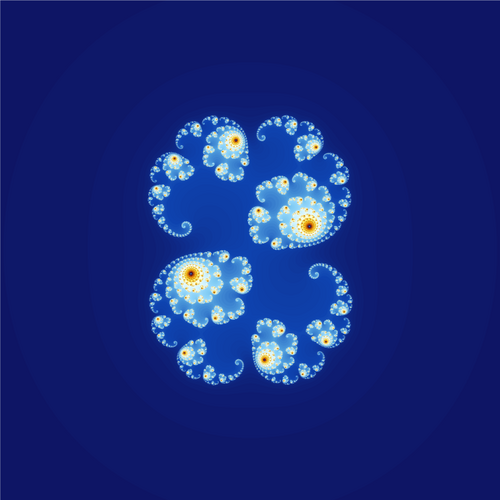
\includegraphics[width=\textwidth]{assets/images/julia-0.285_0.0_-01.png} 
        \caption{Tập Julia $c=0.285+0.0-1i$}
        \label{fig:julia_set_2}

    \end{subfigure}
    \begin{subfigure}[b]{0.3\textwidth}
        \centering
        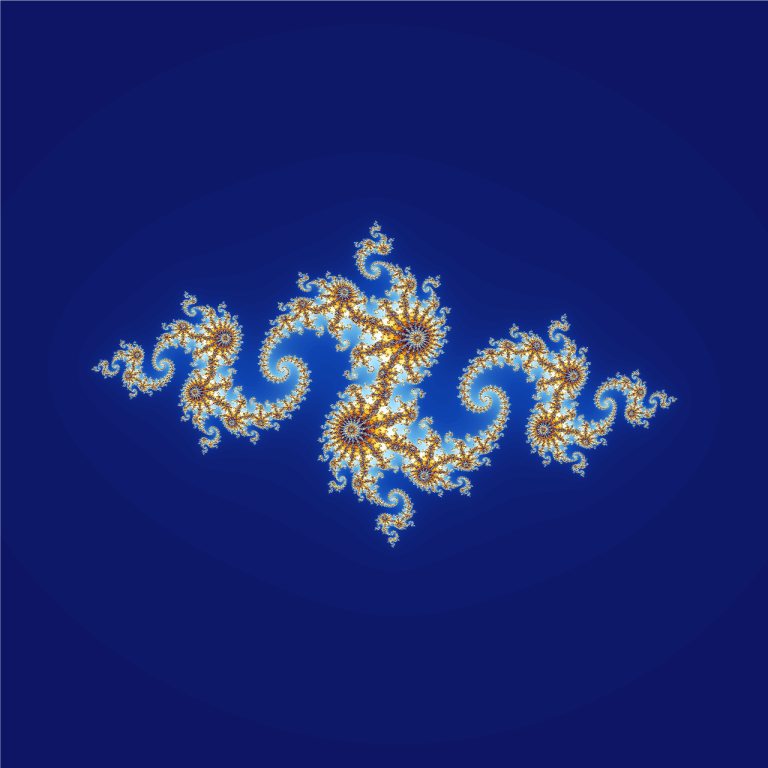
\includegraphics[width=\textwidth]{assets/images/julia_-0.8_0.156.png}
        \caption{Tập Julia $c=-0.8+0.156i$}
        \label{fig:julia_set_3}
    \end{subfigure}
    \begin{subfigure}[b]{0.3\textwidth}
        \centering
        \includegraphics[width=\textwidth]{assets/images/julia_-0.835_-0.2321.png} 
        \caption{Tập Julia $c=-0.835-0.2321i$}
        \label{fig:julia_set_4}
    \end{subfigure}
    \begin{subfigure}[b]{0.3\textwidth}
      \centering
      \includegraphics[width=\textwidth]{assets/images/julia_-0.70176_-0.3842.png} 
      \caption{Tập Julia $c=-0.70176-0.3842i$}
      \label{fig:julia_set_5}
  \end{subfigure}
  \begin{subfigure}[b]{0.3\textwidth}
    \centering
    
\includegraphics[width=\textwidth]{assets/images/Julia_0_0.8.png} 
    \caption{Tập Julia \\ $c=0.0-0.8i$}
    \label{fig:julia_set_6}
  \end{subfigure}
    \caption{Một số hình ảnh tập Julia}
    \label{fig:julia_all}
\end{figure}


\clearpage
\printbibliography

\end{document}